\documentclass[10pt,conference]{IEEEtran}
\IEEEoverridecommandlockouts

\usepackage{cite}
\usepackage{times}
\usepackage{url}
\usepackage[hidelinks]{hyperref}
\usepackage{hypernat}
\usepackage{graphicx}
\usepackage{xcolor}
\usepackage{listings}
\lstset{
  basicstyle=\ttfamily,
  columns=fullflexible,
  frame=single,
  breaklines=true,
  postbreak=\mbox{\textcolor{red}{$\hookrightarrow$}\space},
}

\title{Simulating MPI execution on IITK CSE Cluster}
\author{Yash Srivastav (150839)}

\begin{document}

\maketitle

\section{Problem Description}
MPI programs might behave very differently (in terms of speed) when run on
different host nodes due to the different network arrangement of the nodes.
One might want to test out various different node assignments so as to check
out the impact on data transfer rates / congestion. The target machines should
easily be changeable without having to go through the whole runtime and network
transfers again. Also a simulation might give a better idea independent of real
world factors like load on the CPUs.

\section{Related Work}
A number of works have explored this problem before in order to come up with
solutions to efficiently solve it. There are 2 major ways of tackling this
problem: in-situ (online) simulation and post-mortem (offline) simulation.
In-situ simulators simulate the actual running of the program and while running,
perform necessary calculations / simulations. Port-mortem simulators in general
collect traces during a sample program execution and then simulate the behaviour
later on based on the collected traces.

\cite{netsim} performs in-situ simulation by hooking onto the MPI network layer
and then sending exact packet transfers to network simulator running
simultaneously. Also somehow the computation time itself has to be simulated
while running which requires applying a uniform slowdown to account for latency
introduced due to the network simulator. A benefit of using this method is that
the implemented simulator only needs to simulate packets and doesn't need to
worry about internal algorithms being used.

\cite{time-independent-trace-sim} and \cite{better-sim-ethernet} perform
post-mortem simulations. They both collect traces of \texttt{MPI} events
occurring during the execution and then simulate the behaviour based on the
collected logs. A benefit of using this method is that long computations can be
avoided during simulation as only the expected delay needs to be noted and not
really executed.

\cite{smpi} and \cite{smpi-online} follow a hybrid approach and simulate on a
complete reimplementation of the \texttt{MPI} Standard on the \textbf{SimGrid}
simulation kernel.

The offline approaches employ either simpler network models or use older network
simulation frameworks like \textbf{OmNet++}.

\section{Methodology}
The method we apply in this paper is an offline approach similar to
\cite{time-independent-trace-sim}. The program is run with the \texttt{PMPI}
interface active so as to obtain event traces of \texttt{MPI} events. Also
\textbf{P}erformance \textbf{API} (PAPI) is used to measure the computation
cycles between successive \texttt{MPI} events. This effectively gives us a log of events
which need to be simulated. Something like the following:
\begin{lstlisting}[frame=single]
[0] compute 18288
[0] send 1024 to 1
[1] compute 3108
[1] recv 1024 from 0
[1] compute 29708
[0] compute 127451
[0] wrapping up
[1] wrapping up
\end{lstlisting}

With the above information, its possible to actually simulate these events now
on a network simulator. For this paper, we use the \texttt{ns3} simulation
framework \cite{carneiro2010ns}. Each ranked process is treated as an
application running on a node in the simulator and then simulates itself
accordingly. At the end, we can obtain the total time taken till all
applications reached end of execution as the simulation time.

\section{Implementation Details}
There are two main components to the simulation described in this paper: The
\textbf{Profiler (Trace Collector)} and the \textbf{Simulator}.
\subsection{Profiler (Trace Collector)}
The profiler is a pretty simple PMPI wrapper which allows adding hooks to every
MPI function call before and after execution. Every process in an execution
writes to a log file named \texttt{simpi-\$rank.log}. At the start of every MPI
function, the current instruction count is recorded and a difference from the
previous value is taken and logged. This gives a fair idea of computation
between 2 MPI function calls. This can be used as a measure of delay to be
introduced while simulating. Also every MPI function call itself is logged via
the important params being logged. Right now, the following functions are being
traced and observed:
\begin{itemize}
  \item \texttt{MPI\_Init}: Also used to initialize profiler variables like
    logfile file pointer.
  \item \texttt{MPI\_Finalize}: Close file pointer and any other wrapping up
    needed.
  \item \texttt{MPI\_Send}
  \item \texttt{MPI\_Recv}
  \item \texttt{MPI\_Scatter}
  \item \texttt{MPI\_Gather}
  \item \texttt{MPI\_Bcast} (short message algorithm only)
  % \item \texttt{MPI\_Reduce}
  % \item \texttt{MPI\_Allgather}
  % \item \texttt{MPI\_Allreduce}
  % \item \texttt{MPI\_Alltoall}
\end{itemize}

The implementation only supports a single communicator
\texttt{MPI\_COMM\_WORLD}. Its possible to add support for communicators by
logging the respective calls and then performing computation regarding which
nodes receive which message based on that.

The implementation doesn't care about the result of any of the calls and only
logs the called params. If needed, we could log the results as well.

The profiler compiles to a dynamic library and which can then be specified in
\texttt{LD\_PRELOAD} and then any MPI program executed would be profiled and
traced as needed. Sample trace collection:
\begin{lstlisting}[frame=single]
$ export LD_PRELOAD=$HOME/papi-install/lib/libpapi.so:$HOME/mpich/lib/libsimpi.so
$ mpirun -np 2 ./asgn1-1.x 1
[0] compute 18304
[1] compute 3124
[0] send 1024 to 1
[1] recv 1024 from 0
[1] compute 29665
[0] compute 177282
[0] wrapping up
[1] wrapping up
Runtime = 0.000067
$ cat *.log
0 1 18305
0 3 1024 1
0 1 31557
1 1 3124
1 2 1024 0
1 1 29664
\end{lstlisting}


\subsection{Simulator}
The simulator consists of various different modules:
\begin{itemize}
  \item Parser
  \item Topology Generator
  \item \texttt{MPINode}
\end{itemize}

Sample simulator run:
\begin{lstlisting}[frame=single]
$  ./run-simulator.sh 16 ./test/test-hostfile ./test/test-logs-16
+0.023341061s
\end{lstlisting}

\subsection{Topology Generator}

\begin{figure}
  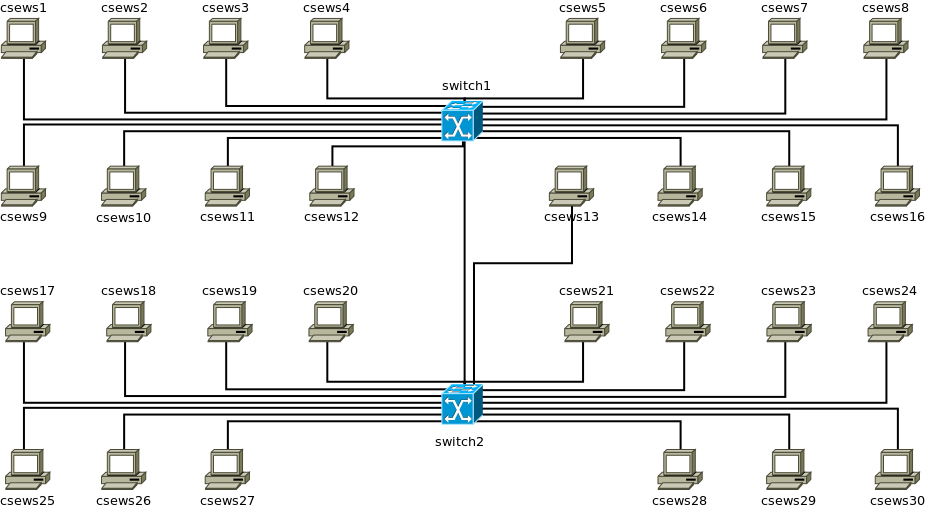
\includegraphics[width=\linewidth]{topology}
  \caption{ CSE Cluster Topology }
  \label{fig:1}
\end{figure}

Generates a topology exactly as per the CSE Cluster as shown in Figure
\ref{fig:1}. Every link is a 1Gbps Connection with CSMA. The two switches are
actually \texttt{ns3::Bridge} in ns3 terminology connected to each other via a
link having the same specifications.

\subsection{Parser}
The parser parses event logs generated by the tracer and creates a rank to events
mapping. Every event in this mapping consists only of the following events:

\begin{itemize}
  \item Compute
  \item Recv
  \item Send
\end{itemize}

All other traced events are converted to a mixture of these as per the
respective algorithms implemented in MPICH 3.2.1.

\subsection{\texttt{MPINode}}
An \texttt{ns3::Application} which is essentially a TCP server + client. Runs on
a host node as per host allocation. Takes as initialization parameters the
following values:
\begin{itemize}
  \item Rank (\texttt{uint16\_t}): The rank of this process as per the global
    rank allocation. Used to determine host allocation of the process.
  \item Events (\texttt{vector<simpi\_event\_tagged\_t>}): A list of events
    supposed to be simulated on this ranked process.
    \texttt{simpi\_event\_tagged\_t} is custom defined type which can be either
    a \textbf{Compute} event or a \textbf{Recv} event or a \textbf{Send} event.
    These are the only three events supported by the \texttt{MPINode} itself.
  \item Addresses (\texttt{vector<Address>}): A list of addresses of every host
    on which the \texttt{MPI} program is being run.
\end{itemize}

Events are processed sequentially as soon as the previous one finishes. Once
there are no more events left, the application is stopped. Once all applications
stop we can claim that the simulation has ended.

If a Compute event is encountered, the application is scheduled to process the
next step after a delay corresponding to \texttt{num\_instructions /
  MPI\_NODE\_CPU\_IPS}. \texttt{MPI\_NODE\_CPU\_IPS} is the number of instructions
processed per second by the host CPU. I am using the value of \textbf{BogoMIPS}
from \texttt{lscpu}. 

If a Recv event is encountered, the node starts listening on a fixed port
calculated from \texttt{rank / ppn}. It accepts any connection and keeps
reading from the accepted socket till the required size has been read.

If a Send event event is encountered, the node connects to the address and port
of the target rank \texttt{MPINode}. It sends all possible values via the
socket.

While sending/receiving messages, I have assumed a header area in the packet
other than the main data. The header is just a field containing necessary data
for the packet transfer such as TAG value, etc. The size of the header is
determined by \texttt{MPI\_HEADER\_SIZE}.

While sending/receiving a message from the same network node, we just send a
single byte message (for synchronization) to the target rank. A receiver
simulates an additional delay of \texttt{MPI\_COPY\_DELAY\_US} microseconds for
the memory copy.

% TODO: Fix this
Right now, due to issues with understanding the socket framework of ns3, there
is an issue when there is a lot of contention on a single link.

\section{Experimental Results}
\subsection{Experimental Setup}
The target programs are run 10 times on the CSE Lab Cluster (Intel(R) Core(TM)
i7-8700 CPU @ 3.20GHz with 1Gbps links) and then once on the simulator. The
predicted time as per the simulator is compared against the average runtime of
the 10 programs. The values of various important variables used during the
simulation are given below:

\begin{center}
  \begin{tabular}{ |c|c| }
    \hline
    Variable & Value \\
    \hline
    \texttt{MPI\_NODE\_PPN} & 8 \\
    \texttt{MPI\_NODE\_LINK\_MTU} & 1460 \\
    \texttt{MPI\_NODE\_CPU\_IPS} & 6384000000 \\
    \texttt{MPI\_COPY\_DELAY\_US} & 20 \\
    \texttt{MPI\_HEADER\_SIZE} & 20 \\
    \hline
  \end{tabular}
\end{center}

All programs are executed with \texttt{nprocs=64}.

\subsection{Results}
The comparison between actual runtimes and simulated runtime for simple
testcases is in Figure \ref{fig:2}.

\begin{figure}
  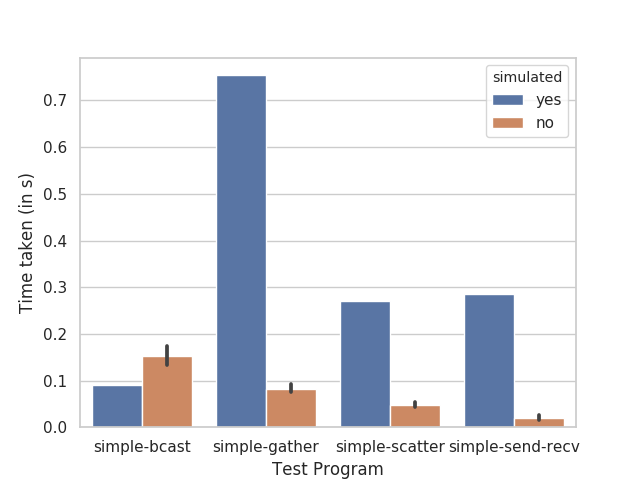
\includegraphics[width=\linewidth]{plot}
  \caption{ Simulation vs Actual }
  \label{fig:2}
\end{figure}

\section{Future Work}
The following can be done to improve the current implementation:
\begin{itemize}
  \item Add support for different communicators.
  \item Add support for handling \texttt{MPI} function errors during tracing and
    logging them as well for use during simulation.
  \item Remaining collectives and Async variants of \texttt{MPI} functions and
    associated calls like \texttt{MPI\_Wait}
  \item Vector variants of \texttt{MPI} collectives (like
    \texttt{MPI\_Allgatherv})
  \item Allow greater send and receive sizes (fix socket + packet sending
    issue).
  \item Comparison with other \texttt{MPI} simulation frameworks developed as
    part of other works.
  \item Distributed trace collection: The trace collection itself could be run
    parallelly on multiple machines for faster trace collection and simulation.
\end{itemize}

\section{Conclusions}
The above results show that simulation is a viable option for predicting
performance of MPI program. Once most operations are implemented, its possible
to use this for actually simulating any MPI program.

\bibliographystyle{IEEEtran}
\bibliography{paper}

\end{document}

